\documentclass[]{article}
\usepackage{nips13submit_e,times}
\usepackage[utf8x]{inputenc}
\usepackage{amsfonts}
\usepackage{indentfirst}
\usepackage{hyperref}
\usepackage{graphicx}
\usepackage{enumerate}
\usepackage{amsmath}
\usepackage{subfigure}
\usepackage{amsopn}
\title{Project-II by group TORONTO}
\author{Michalina Pacholska \And Jakub Sygnowski}
\nipsfinalcopy


\begin{document}

\section{Persons recognition}
\subsection{Problem and dataset descriptions}
  During the project, we were first given a set images and labels indicating if there is a person. We also were given features extracted from the images and we are supposed to analyze and learn our algorithms only on those extracted features (not on images). Then, a week before the deadline, we were given a test set of features for which we should give our predictions. (Following discussions refer to the train set of features). 

  Our set contains $8545$ images and labels ($1$ - person, $0$ - not), and for every image $9360$ features in a form of a $26\times10\times36$ cube. There are $1237$ images with a person (at least labeled $1$). 

\begin{figure}[!h]
  \center
  \subfigure[picture]{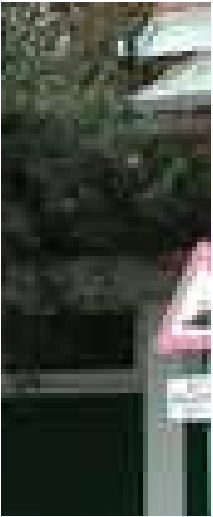
\includegraphics[height=1.7in]{../figures/examplePicture-crop.pdf} \label{fig:examplePicture}}
  \;
  \subfigure[features]{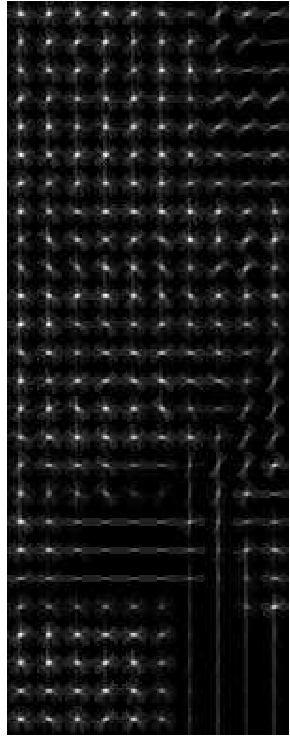
\includegraphics[height=1.7in]{../figures/exampleFeature-crop.pdf} \label{fig:exampleFeature}}
  \caption{ \ref{fig:examplePicture} picture No 200 and \ref{fig:exampleFeature} features extracted form it, using Piotr's toolbox (http://vision.ucsd.edu/~pdollar/toolbox/doc/index.html) %TODO where put this reference
  }
\end{figure}

\subsection{Data analysis and preparation}
  Features first two dimensions $26\times10$ of features for particular image correspond to the position of image form where those features1 were extracted and in the third dimension corresponds to the direction of edges in that part of image. White color and big number indicates that there is the edge, see \ref{fig:examplePicture} and \ref{fig:exampleFeature}. Values of features are between $0$ and $0.2$ and normalization doesn't change them much. 
  \begin{figure}[!h]
  \center
  \subfigure[original data]{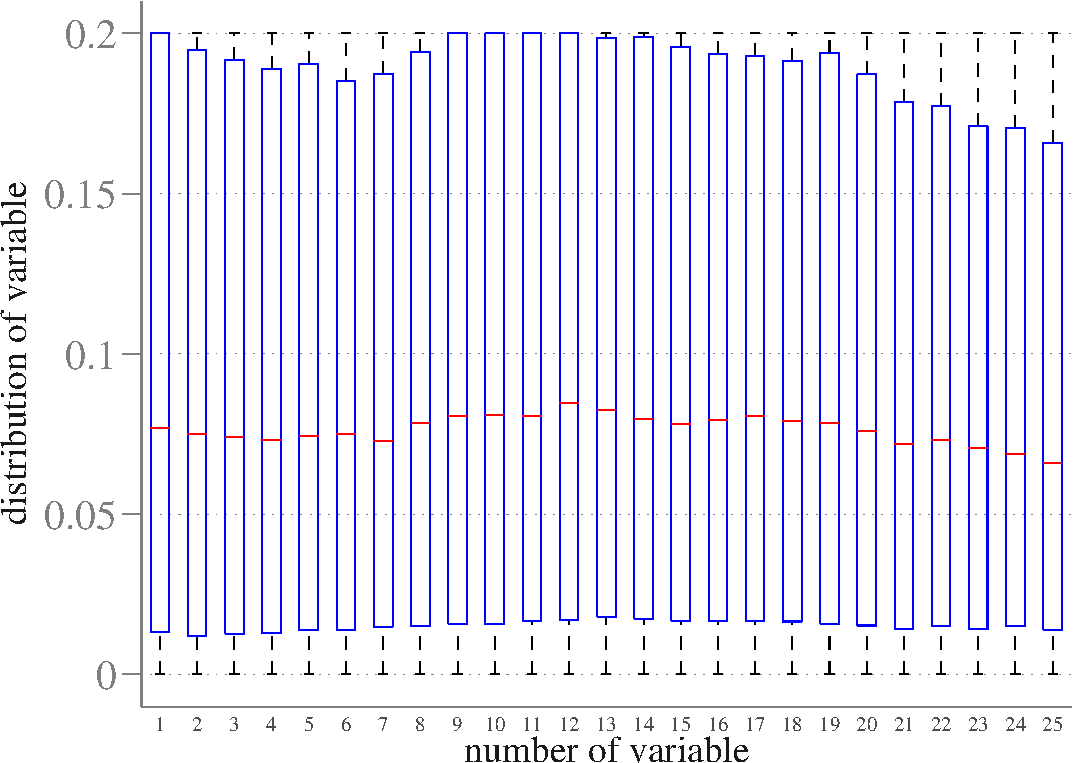
\includegraphics[height=1.8in]{../figures/boxplot1-crop.pdf} \label{fig:boxplot1}}
  \;
  \subfigure[after normalization]{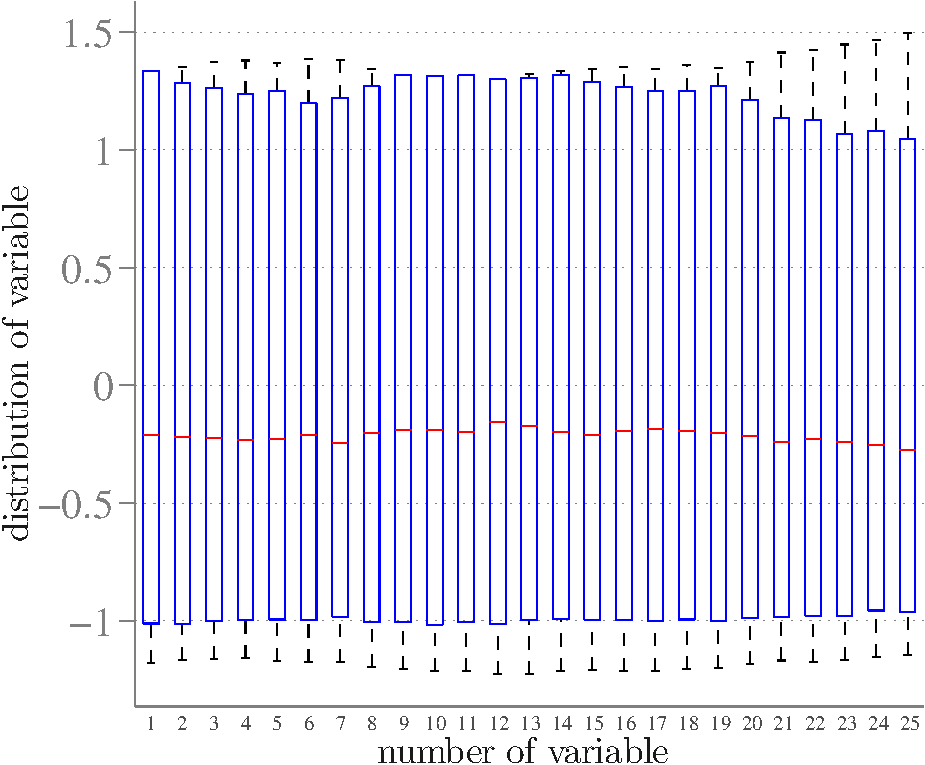
\includegraphics[height=1.8in]{../figures/boxplot2-crop.pdf} \label{fig:boxplot2}}
  \caption{Boxplots of part of the data before \ref{fig:boxplot1} and after \ref{fig:boxplot2} normalization. Rest of the data looks similar.}
\end{figure}
  
  Since there are $9360$ numbers for one picture using all of them will cause overfitting (there is more features than pictures). We calculated correlation of them with output and we obtained picture of abstract person, see \ref{fig:correlation}.
  Also on figure \ref{fig:correlations} we can see that there are regions and gradient more and less important for this task and they have shape of a person. Values of correlation were between $-0.37$ and $0.37$
  \begin{figure}[t]
    \center
    \subfigure[Absolute value of correlation for different directions of gradient]{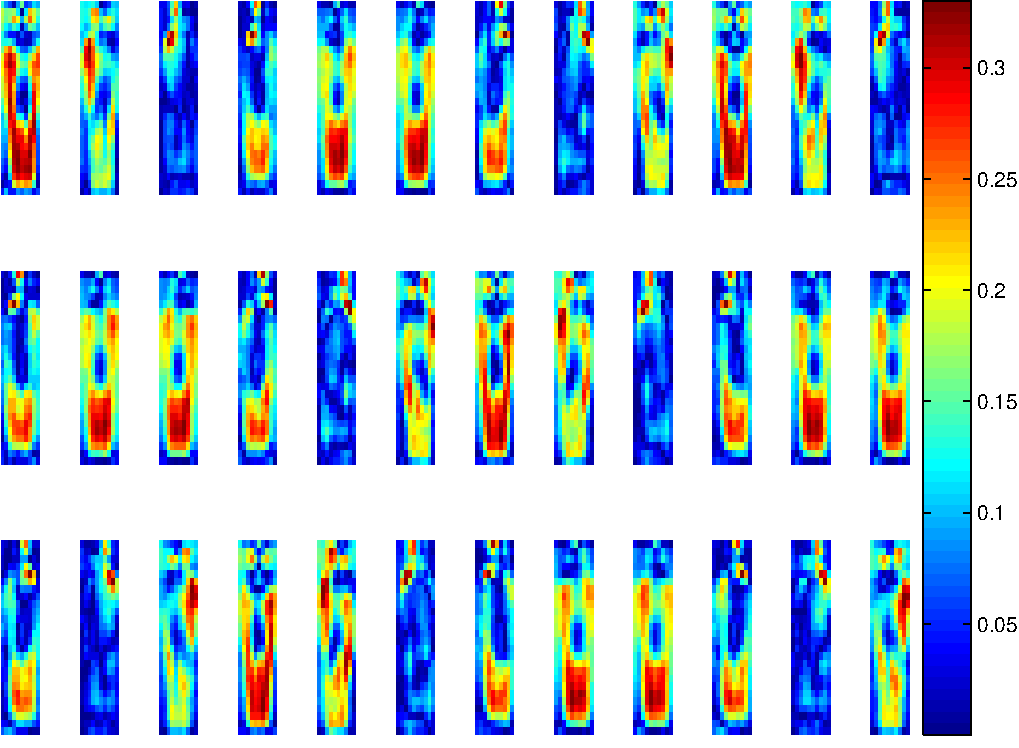
\includegraphics[height=1.7in]{../figures/absoluteCorelation-crop.pdf} \label{fig:correlations}}
      \;\;\;
    \subfigure[positive correlation]{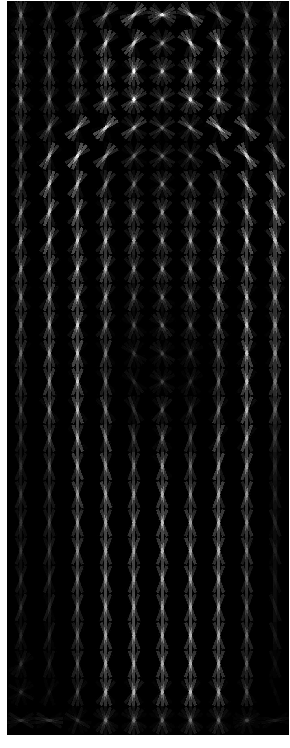
\includegraphics[height=1.7in]		{../figures/averagePerson-crop.pdf} \label{fig:correlation}}
    \caption{Absolute value \ref{fig:correlations} and only positive part \ref{fig:correlation} of correlation, plotted as a feature. There is a lot of not correlated data (deep blue).}
  \end{figure}
  
  Other way of shrinking amount of features is singular value decomposition (i.e. taking only some vectors corresponding to the biggest singular values). That is probably better idea, because correlation captures only linear dependence and don't see structure in the data. We did $SVD$ for $1000$ singular values, and then used $8545\times1000$ as our new feature matrix for testing different methods.
   
% TODO: test matrices descriptions.

\section{Applied methods}
We applied many methods for this task, for most of them we used existing libraries. To check which method is better we were were doing cross-validation and then taking predictions both for train and test into one big vector and passing it as predictions to function \verb+evaluateMultipleMethods+, which was given to us together with data. That was giving us estimate how big is estimate of particular method.

\subsection{Penalized logistic regression}
We started with the the simplest (penalized) logistic regression. Not surprisingly, this method has quite big bias. What's interesting, when we were using $1000$ features (from $SVD$) it also had big variance. Setting bigger penalty ($\lambda$) caused even bigger bias and very poor performance. Decreasing number of features helped decreasing variance. Penalized logistic regression was working the best with only about $120$ features and $\lambda = 0.1$, see \ref{fig:ROClinear}.
% [p1,p2,y] = crossValidation(labels(permutacja),U(permutacja,1:120),4,0.1);
  \begin{figure}[!h]
    \center
    \subfigure[ROC curves for penalized logistic regression (test and train data) compared with random assignment.]{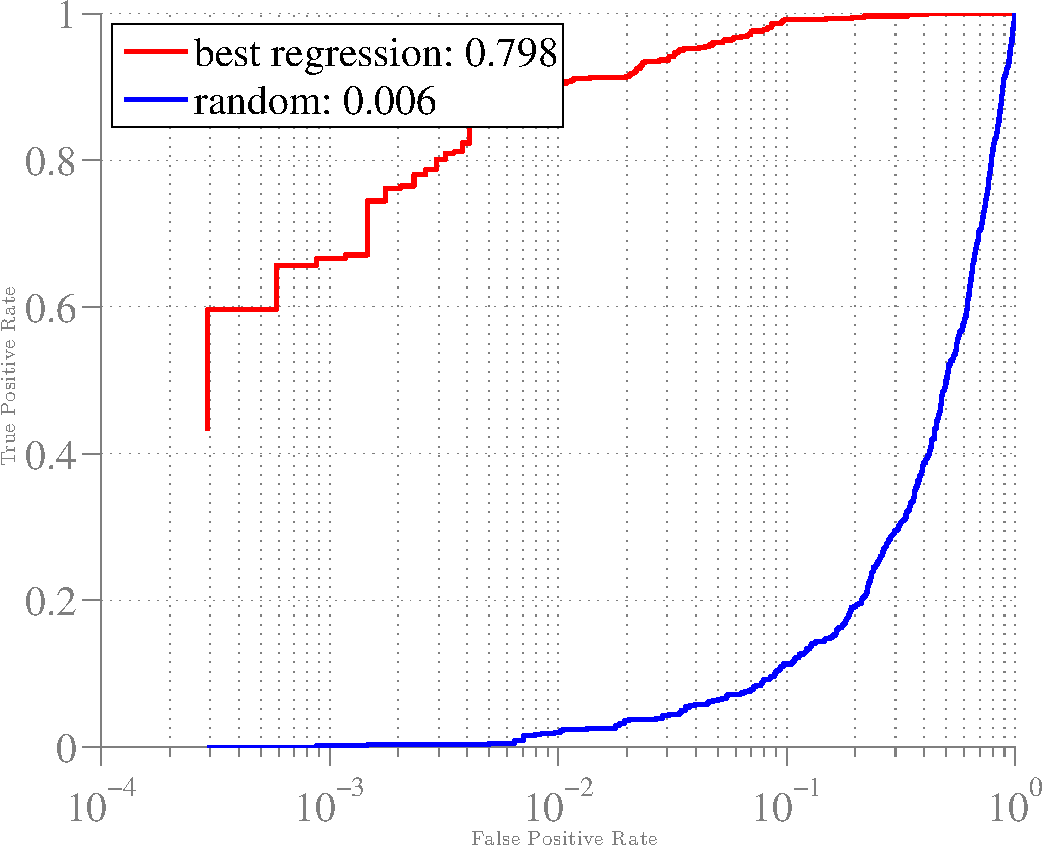
\includegraphics[height=1.7in]{../figures/ROClinear-crop.pdf} \label{fig:ROClinear}}
    \caption{ROC curves...}
  \end{figure}

\subsection{SVM}

\subsection{Neural Network}

\subsection{Random Forest}




\end{document}
